\documentclass[a4paper, 10pt]{article}
\usepackage[utf8x]{inputenc}
\usepackage{graphicx}
\usepackage{geometry}
\usepackage{amsmath}
\usepackage{amssymb}
\usepackage{mathrsfs}
\geometry{hmargin = 2.5cm, vmargin = 1.5cm}

% OPENING
\title{SY09 - TP01\\Statistique descriptive, Analyse en composantes principales}
\author{Bertrand Bon - Antoine Hars}

\begin{document}

\maketitle

L'objectif de ce tp est d'apprendre \`a manipuler une grande quantit\'e de données au moyen d'outils
de statistique descriptive et d'analyse en composantes principales.

\section{Statistique Descriptive}
\subsection{Donn\'ees babies}

Dans cet exercice, nous disposons d'un jeu de donn\'ees \textit{babies} constitu\'e de 1236 b\'eb\'es
d\'ecrits par 23 variables. Dans notre tp, nous n'utilisons que 8 variables : 5 quantitatives
(le poids \`a la naissance, la dur\'ee de gestation, le nombre de grossesses pr\'ec\'edentes,
la taille de la m\`ere et le poids de la m\`ere) et 3 qualitatives (l'\^age de la m\`ere,
si la m\`ere fume ou non et le niveau d'\'education de la m\`ere).\\
% QUESTION
\newline\textbf{Quelle est la différence de poids entre les bébés nés de mères qui fumaient durant leur grossesse et celles
qui ne fumaient pas ?}\\
Pour observer cette différence, nous pouvons étudier le résumé des valeurs du poids des b\'eb\'es en fonction du fait
que leur m\`ere fumait ou non :\\ \\
\begin{tabular}{|c|c|c|c|c|c|c|}
\hline
Min & 1st Qu. & Median & Mean & 3rd Qu. & Max \\
\hline
58.0 & 102.0 & 115.0 & 114.1 & 126.0 & 163.0 \\
\hline
\end{tabular}\\
\textit{R\'esum\'e des valeurs des b\'eb\'es n\'es d'une m\`ere fumeuse}\\ \\
\begin{tabular}{|c|c|c|c|c|c|c|}
\hline
Min & 1st Qu. & Median & Mean & 3rd Qu. & Max \\
\hline
55.0 & 113.0 & 123.0 & 123.0 & 134.0 & 176.0 \\
\hline
\end{tabular}\\
\textit{R\'esum\'e des valeurs des b\'eb\'es n\'es d'une m\`ere non fumeuse}\\ \\
\`A travers ces deux tableaux, nous pouvons observer une diff\'erence entre les deux populations :
Suivant la moyenne et la m\'ediane des deux tableaux de donn\'ees, il semble que les enfants de mère fumeuse
ont tendance \`a na\^itre plus maigres que ceux d'une m\`ere non fumeuse.\\ \\
Pour v\'erifier cette tendance, nous pouvons observer le graphique suivant :\\
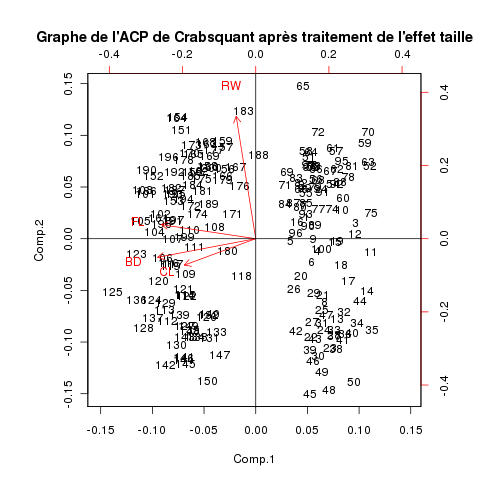
\includegraphics[height = 8cm, width = 8cm]{plots/boxplot_bwt_smoke.png}\\ \\
L'observation de ce boxplot nous permet de confirmer la tendance observ\'ee.
De plus, nous pouvons constater une pr\'esence plus importante de valeurs atypiques chez les m\`eres fumeuses.\\
Les intervalles de confiance pour les deux m\'edianes ne se chevauchent pas donc les deux m\'edianes diff\'erent et nous pouvons
dire que dans 95\% des cas, la différence de poids est significative.
Un b\'eb\'e d'une m\`ere fumeuse est donc statistiquement plus maigre qu'un b\'eb\'e d'une m\`ere non fumeuse.\\ \\
% QUESTION
\textbf{Est-ce qu'une m\`ere qui fume durant sa grossesse est encline \`a avoir un temps de gestation plus courts qu'une
m\`ere qui ne fume pas ?}\\
Pour répondre à cette question, nous étudions le résumé du temps de gestation en fonction du fait
que la m\`ere fumait ou non :\\ \\
\begin{tabular}{|c|c|c|c|c|c|c|}
\hline
Min & 1st Qu. & Median & Mean & 3rd Qu. & Max\\
\hline
223.0 & 271.0 & 279.0 & 278.0 & 286.0 & 330.0\\
\hline
\end{tabular}\\
\textit{R\'esum\'e des valeurs du temps de gestation d'une m\`ere fumeuse}\\ \\
\begin{tabular}{|c|c|c|c|c|c|c|}
\hline
Min & 1st Qu. & Median & Mean & 3rd Qu. & Max\\
\hline
148.0 & 273.0 & 281.0 & 280.2 & 289.0 & 353.0\\
\hline
\end{tabular}\\
\textit{R\'esum\'e des valeurs du temps de gestation d'une m\`ere non fumeuse}\\ \\
Nous pouvons observer que les m\'edianes sont l\'eg\`erement diff\'erentes ce qui nous permet de dire que le fait de fumer peut conduire \`a
une modification sur la gestation mais il n'est pas possible d'établir clairement ce point avec les deux r\'esum\'es.\\ \\
Nous avons ensuite observ\'e les deux populations au moyen d'un boxplot :\\
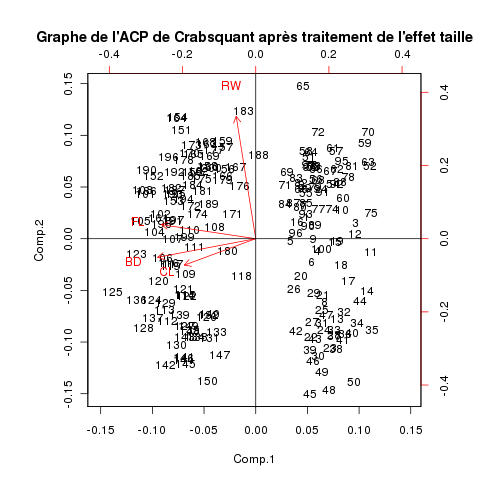
\includegraphics[height = 8cm, width = 8cm]{plots/boxplot_gestation_smoke.png}\\
Concernant ce graphique, il est apparu que du cot\'e des femmes ne fumant pas, il y avait un nombre cons\'equent de valeurs atypiques.
Afin d'\'etudier ce boxplot au niveau des m\'edianes et des intervalles de confiance, nous n'affichons pas
ces valeurs atypiques sur ce graphique.\\
Ce graphique nous montre que les intervalles de confiance des m\'edianes se chevauchent, donc il n'est pas possible depuis ce graphique de
dire si oui ou non les m\`eres ne fumant pas ont un temps de gestation plus long que des m\`eres fumeuses.\\ \\
% QUESTION
\textbf{Le niveau d'\'etude a-t-il une influence sur le fait que la m\`ere soit fumeuse ?}\\
Afin de r\'epondre \`a cette question, nous \'etudions dans un premier temps le tableau de contingence des donn\'ees :\\ \\
\begin{tabular}{|c|c|c|c|c|c|c|c|}
\hline
 & 0 & 1 & 2 & 3 & 4 & 5 & 7\\
\hline
M\`eres non fumeuses & 15 & 79 & 264 & 30 & 194 & 154 & 6 \\
\hline
M\`eres fumeuses & 4 & 102 & 176 & 33 & 102 & 65 & 1 \\
\hline
\end{tabular}\\
\textit{Tableau de contingence du niveau d'étude des mères}\\ \\
L'\'etude de tableau de contingence nous apporte des \'eclaircissements sur plusieurs points :\\
Nous pouvons affirmer qu'il y a de grande diff\'erences pour chaque classe d'\'etude si un m\`ere fume ou pas.
Ce tableau ne prend pas en compte le niveau d'\'etude n°6 puisqu'aucune m\`ere des deux populations n'en fait partie.\\ \\
Concernant les niveaux d'\'etude 2, 4 et 5 (les niveaux avec le plus grand \'ecart de valeurs), le nombre de m\`eres varie beaucoup
suivant le fait qu'elles fument ou non.\\ \\
Nous pouvons ensuite observer les deux populations de m\`eres au moyen d'un barplot :\\
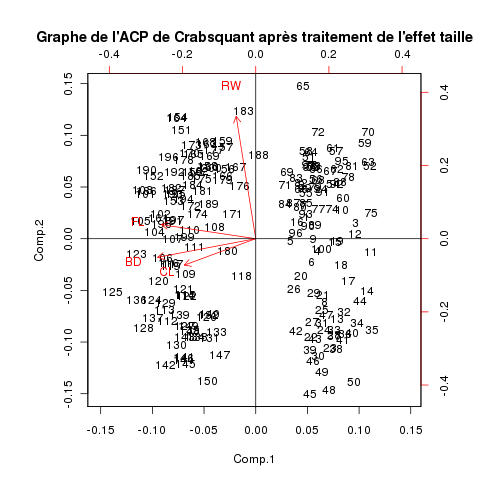
\includegraphics[height = 8cm, width = 8cm]{plots/barplot_etude_smoke.png}\\
Ce barplot illustre le tableau de contingence et montre que pour les niveaux d'\'etude 2, 4 et 5, il y a une plus grand proportions de
m\`eres non fumeuses alors quand le cas du niveau d'\'etude 1, le nombre de m\`eres fumeuses et plus grand que celui
des m\`eres non fumeuses.\\ \\
L'\'etude pr\'esent\'ee nous montre que les femmes non fumeuses sont moins propices \`a avoir un enfant avec un faible poids à la naissance
que les femmes qui fument, ce qui correspond à nos analyses.\\
Du cot\'e de l'\'etude pr\'esent\'ee, il est expliqu\'e qu'il n'y a pas de lien entre le fait de fumer et le temps de gestation des femmes.
De notre cot\'e, nous avons pu observer une l\'eg\`ere diff\'erence entre les donn\'ees des m\`eres fumeuses et non fumeuses mais ces donn\'ees
ne nous permettent aucunement de d\'eterminer statistiquement l'influence du tabagisme sur ce temps de gestation.\\
Concernant la relation entre le niveau d'\'etude et le tabagisme, nous pouvons dire qu'il semble que les femmes avec un niveau d'\'etude
\'elev\'e fument moins mais il est apparu que sur notre \'echantillon de donn\'ees, les femmes avec un niveau d'\'etude 2 et non fumeuses
sont plus importantes que les femmes du m\^eme niveau et fumeuses donc il est difficile de trouver un lien entre ces deux crit\`eres.

\subsection{Donn\'ees crabs}

Dans cet exercice, nous avons \'etudi\'e un jeu de donn\'ees constitu\'e de 200 crabes d\'ecrits par huits variables
(trois variables qualitatives et cinq quantitatives).\\
Nous pouvons repr\'esenter les variables quantitaives de crabsquant sous la forme du graphique suivant :\\
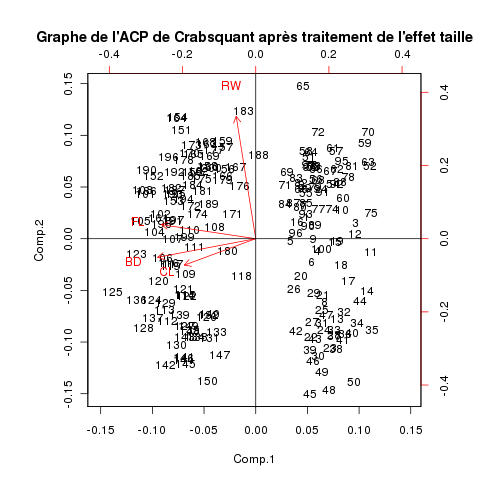
\includegraphics[height = 8cm, width = 8cm]{plots/boxplot_crabsquant.png}\\
Ce graphique nous montre donc un valeur atypique pour la variable \textit{RW} et fait ressortir la pr\'esence de deux groupes de variables
ayant une dispersion similaire entre elles :
les variables \textit{FL}, \textit{RW} et \textit{BD} d'un cot\'e et les variables \textit{CL} et \textit{CW} de l'autre.\\ \\
% QUESTION
\textbf{Existe-t-il des diff\'erences de caract\'eristiques morphologiques selon l'esp\`ece ou le sexe ?
Semble-t-il possible d'identifier l'esp\`ece ou le sexe d'un crabe \`a partir d'une ou plusieurs mesures de ces caract\'eristiques ?}\\
Nous affichons les donn\'ees des crabes en fonction de l'esp\`ece et du sexe des crabes :\\
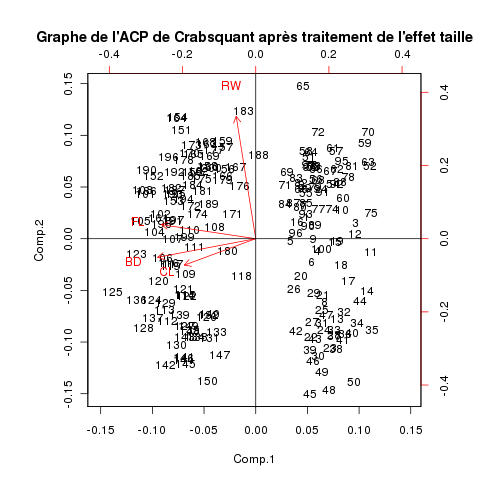
\includegraphics[height = 8cm, width = 8cm]{plots/plot_crabsquant_sp.png}
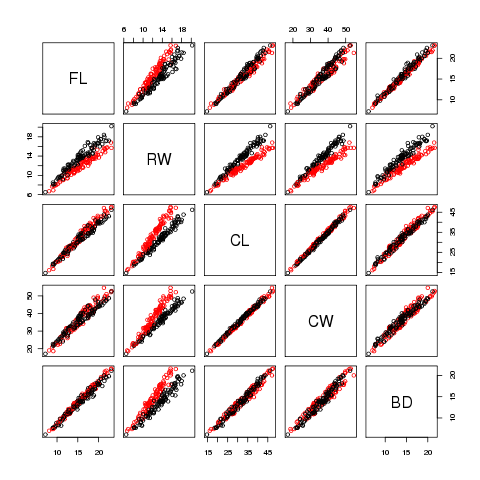
\includegraphics[height = 8cm, width = 8cm]{plots/plot_crabsquant_sex.png}\\
Ces deux graphiques nous montrent qu'il est difficile de d\'eterminer le sexe ou l'esp\`ece d'un crabe \`a partir des variables disponibles.\\
Afin de d\'eterminer l'existence de diff\'erences de caract\'eristiques morphologiques selon l'esp\`ece ou le sexe, nous comparons les donn\'ees
suivantes :\\
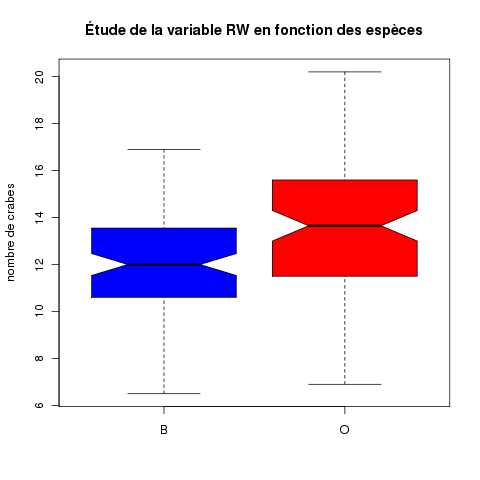
\includegraphics[height = 4cm, width = 3cm]{plots/boxplot_rw_espece.png}
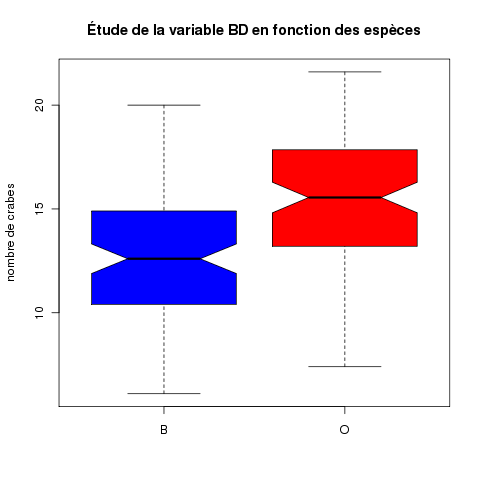
\includegraphics[height = 4cm, width = 3cm]{plots/boxplot_bd_espece.png}
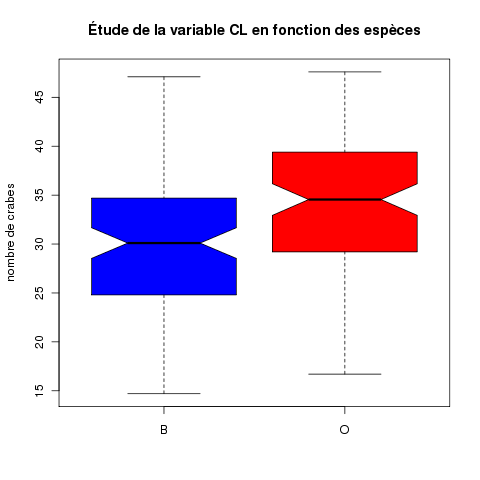
\includegraphics[height = 4cm, width = 3cm]{plots/boxplot_cl_espece.png}
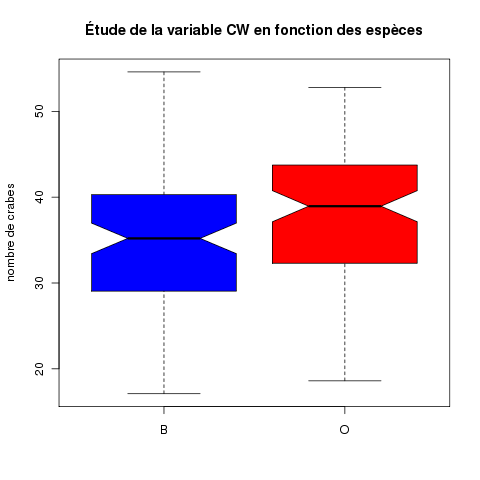
\includegraphics[height = 4cm, width = 3cm]{plots/boxplot_cw_espece.png}
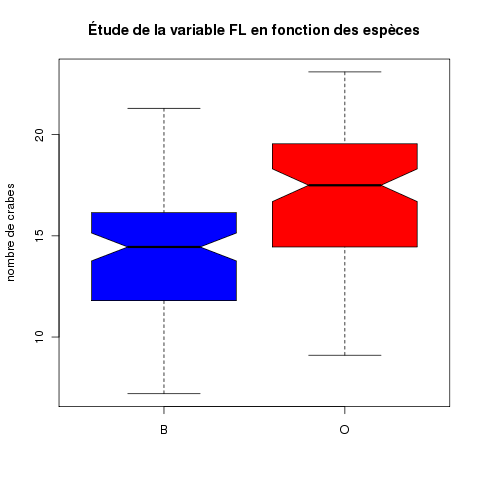
\includegraphics[height = 4cm, width = 3cm]{plots/boxplot_fl_espece.png}\\
En fonction des esp\`eces, nous pouvons voir que toutes les caract\'eristiques diff\`erent.
La dispersion des donn\'ees est par contre similaire pour chaque boxplot.\\ \\
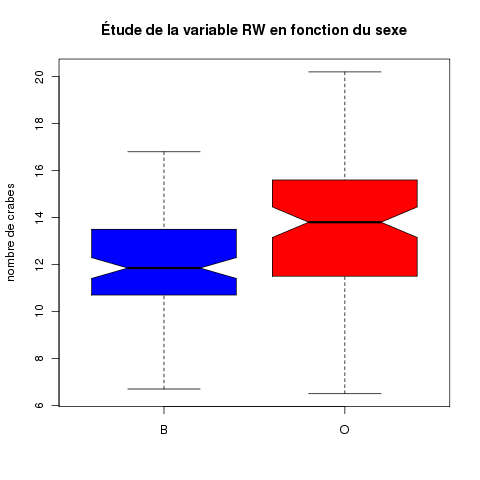
\includegraphics[height = 4cm, width = 3cm]{plots/boxplot_rw_sexe.png}
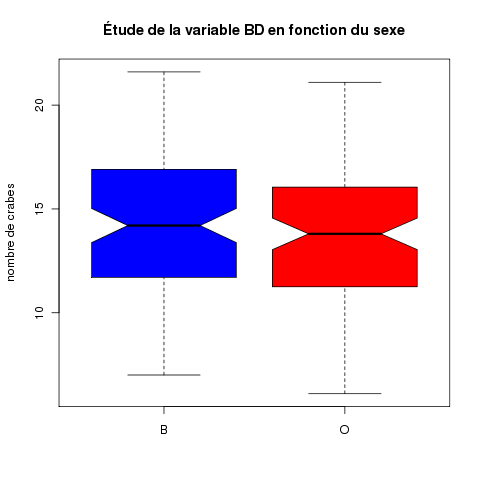
\includegraphics[height = 4cm, width = 3cm]{plots/boxplot_bd_sexe.png}
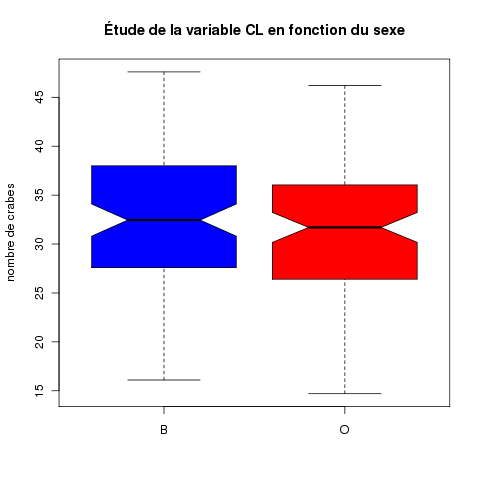
\includegraphics[height = 4cm, width = 3cm]{plots/boxplot_cl_sexe.png}
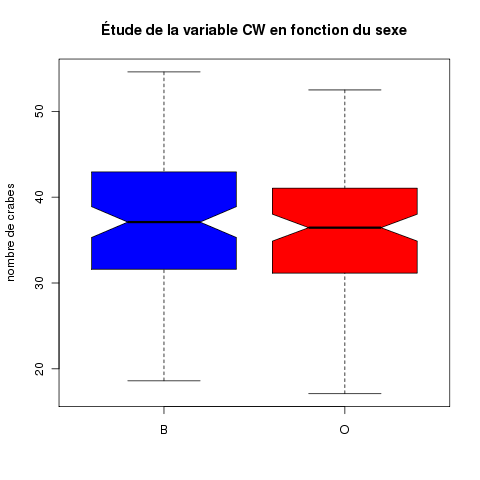
\includegraphics[height = 4cm, width = 3cm]{plots/boxplot_cw_sexe.png}
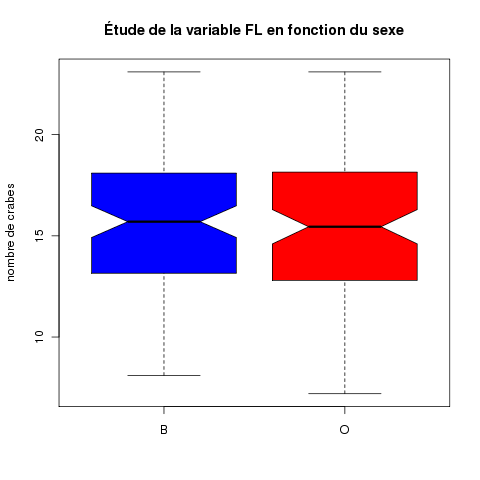
\includegraphics[height = 4cm, width = 3cm]{plots/boxplot_fl_sexe.png}\\
Par rapport au sexe des crabes, nous remarquons que toutes les caract\'eristiques (\`a part \textit{RW}) sont plut\^ot proches au vu
du chevauchement des intervalles de confiance et la dispersion des donn\'ees est environ la m\^eme pour les boxplots.\\ \\
Les crabes \textit{B} ont des valeurs plus \'elev\'ees pour toutes les variables quantitatives.\\ \\ \\ \\ \\
% QUESTION
\textbf{Quelle la cause de la corr\'elation entre les diff\'erentes variables ?
Quel traitement est-il possible d'appliquer aux donn\'ees pour s'affranchir de ce ph\'enom\`ene de corr\'elation ?}\\
On peut voir qu'il existe une forte corr\'elation entre toutes les combinaisons de variables.
Vu qu'il s'agit de mesures de certaines parties du corps des crabes, il est normal que chaque variable soit proportionnelle aux autres.
Le contraire signifierait que les crabes n'ont pas de proportions corporelles harmonieuses.\\ \\
Pour confirmer cette forte corr\'elation, nous calculons les coefficients de corr\'elation :\\ \\
\begin{tabular}{|c|c|c|c|c|c|c|}
\hline
 & FL & RW & CL & CW & BD\\
FL & 1.000 & 0.907 & 0.979 & 0.965 & 0.988\\
\hline
RW & 0.907 & 1.000 & 0.893 & 0.900 & 0.889\\
\hline
CL & 0.979 & 0.893 & 1.000 & 0.995 & 0.983\\
\hline
CW & 0.965 & 0.900 & 0.995 & 1.000 & 0.968\\
\hline
BD & 0.988 & 0.889 & 0.983 & 0.968 & 1.000\\
\hline
\end{tabular}\\
\textit{Tableau des coefficients de corr\'elation entre les variables}\\ \\
La variable la plus corr\'el\'ee est la variable \textit{CL} suite à la somme de ces corr\'elations.
Pour s'affranchir de ce ph\'enom\`ene de corr\'elation, nous pouvons diviser les donn\'ees par cette variable pour d\'ecorr\'eler
les variables.

\section{Analyse en composantes principales}
\subsection{Exercice th\'eorique}

Le but de cette partie est de comprendre l'ACP, une analyse permettant de traiter des donn\'ees multi-dimensionnelles d'un espace
large de variables en r\'eduisant celui-ci.
\[M =
\begin{pmatrix}
3 & 4 & 3\\
1 & 4 & 3\\
2 & 3 & 6\\
2 & 1 & 4
\end{pmatrix}\]\\
% QUESTION
\textbf{Calcul des axes factoriels de l'ACP du nuage d\'efini}\\
Pour obtenir les axes factoriels, on centre la matrice :
\[M' =
\begin{pmatrix}
1 & 1 & -1\\
-1 & 1 & -1\\
0 & 0 & 2\\
0 & -2 & 0
\end{pmatrix}\]
puis on calcule la matrice de variance :
\[S = \frac{1}{n}.M'.M = \frac{1}{4}.M'.M =
\begin{pmatrix}
0.5 & 0 & 0\\
0 & 1.5 & -0.5\\
0 & -0.5 & 1.5
\end{pmatrix}\]
En diagonalisant cette matrice, nous obtenons les valeurs propres et les axes d'inertie suivants :\\ \\
\begin{tabular}{|c|c|c|c|}
\hline
 & $\lambda1$ & $\lambda2$ & $\lambda3$\\
\hline
valeurs propres & 2.0 & 1.0 & 0.5\\
\hline
\% axes d'inertie & 57.14 & 28.57 & 14.29\\
\hline
\% axes d'inertie cumul\'es & 57.14 & 85.71 & 100.0\\
\hline
\end{tabular}\\ \\
Nous pouvons remarquer que les deux premiers axes cumulent environ 86\% de l'information.
Donc nous pouvons repr\'esenter 86\% de l'information sur le plan factoriel d\'efini par les deux premiers axes.\\
Le calcul des composantes principales donne la matrice :\\
\[C =
\begin{pmatrix}
-1.41 & 0 & 1\\
-1.41 & 0 & -1\\
1.41 & 1.41 & 0\\
1.41 & -1.41 & 0
\end{pmatrix}\]
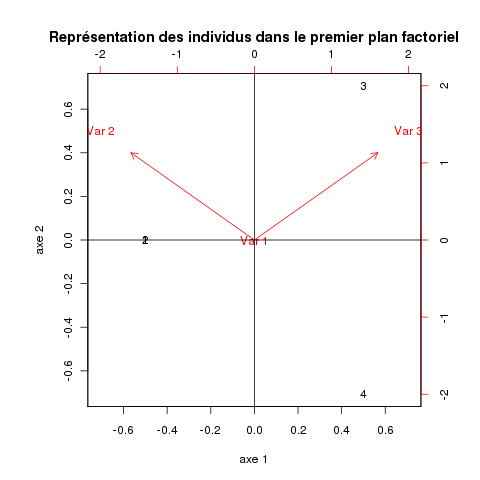
\includegraphics[height = 8cm, width = 8cm]{plots/plot_composantes_principales.png}\\
Sur ce graphique, nous pouvons observer que les deux premiers individus correspondent au m\^eme point dans le premier plan factoriel
et que la seule coordonn\'ee qui peut diff\'erencier ces deux points d\'epend du troisi\`eme axe factoriel.\\ \\
% QUESTION
\textbf{Traçage de la repr\'esentation des trois variables dans le premier plan factoriel}\\
On calcule les corr\'elations entre les variables pour avoir leurs coordonn\'ees sur le premier plan factoriel :\\
\[D = cor(M', C) =
\begin{pmatrix}
0 & 0 & 1\\
-0.816 & 0.577 & 0\\
-0.816 & 0.577 & 0
\end{pmatrix}\]
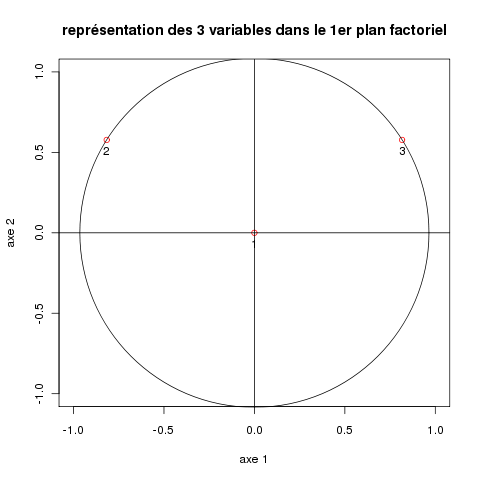
\includegraphics[height = 8cm, width = 8cm]{plots/plot_correlation.png}\\
% QUESTION
\textbf{Calcul de l'expression $\mathbf{\sum_{\alpha=0}^n c_{\alpha}.u'_{\alpha}}$ pour les valeurs \textit{k =} 1, 2 et 3}\\ \\
$k = 1 :
\begin{pmatrix}
0 & 1 & -1\\
0 & 1 & -1\\
0 & -1 & 1\\
0 & -1 & 1
\end{pmatrix}$,
$k = 2 :
\begin{pmatrix}
0 & 1 & -1\\
0 & 1 & -1\\
0 & 0 & 2\\
0 & -2 & 0
\end{pmatrix}$,
$k = 3 :
\begin{pmatrix}
1 & 1 & -1\\
-1 & 1 & -1\\
0 & 0 & 2\\
0 & -2 & 0
\end{pmatrix} = M'$\newpage

\subsection{Utilisation des outils R}
% QUESTION
\textbf{Effectuer l'ACP du jeu de donn\'ees notes \'etudi\'e en cours. Montrer comment on peut retrouver tous les r\'esultats alors
obtenus (valeurs propres, axes principaux, composantes principales, repr\'esentations graphiques)}\\
On calcule l'ACP avec l'instruction : \textit{acp = princomp(notes)}\\
On obtient les axes d'inertie et axes d'inertie cumul\'es avec l'instruction \textit{summary(acp)}\\
La matrice des composantes principales est contenue dans la variable \textit{acp\$scores}\\
Les vecteurs propres sont obtenue dans la variable \textit{acp\$loadings}\\
On établit le graphique de la repr\'esentation des individus :\\
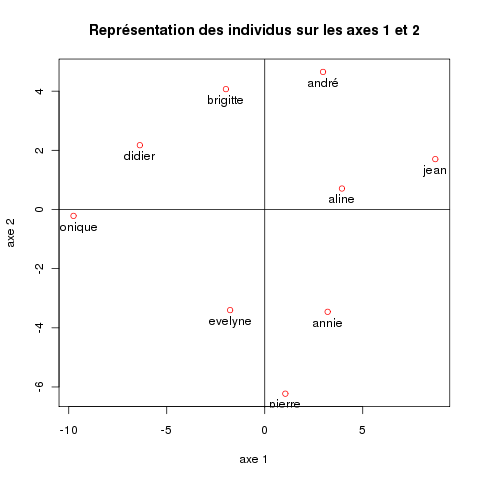
\includegraphics[height = 8cm, width = 8cm]{plots/plot_acp_notes.png}\\
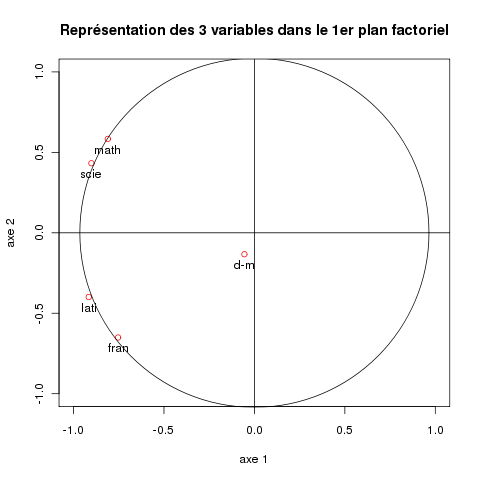
\includegraphics[height = 8cm, width = 8cm]{plots/plot_correlation_notes.png}
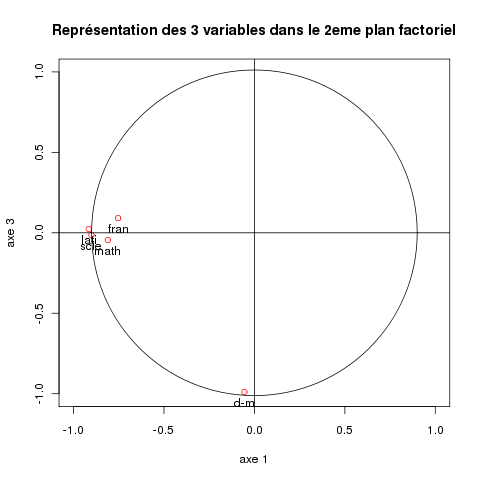
\includegraphics[height = 8cm, width = 8cm]{plots/plot_correlation_notes_2.png}\\ \\
% QUESTION
\textbf{Qu'affichent les fonctions \textit{plot} et \textit{biplot} ?}\\
La fonction \textit{princomp} r\'ealise l'ACP sur la matrice et nous retourne l'\'ecart-type pour la valeur \textit{sdev}.
La valeur \textit{loadings} nous permet d'avoir les axes factoriels, c'est-\`a-dire les vecteurs propres de la matrice de variance.
La valeur \textit{scores} nous donne la matrice des composantes principales.\\ \\
L'utilisation de la fonction \textit{plot} sur le r\'esultat de \textit{princomp} affiche les valeurs propres associ\'ees \`a chaque composante.\\
La fonction \textit{biplot} permet de projeter les individus et les variables sur un m\^eme plan.
Il est utile d'utiliser cette fonction pour \'evaluer graphiquement les corr\'elations entre les variables (par rapport \`a l'angle que forment
deux vecteurs). Deux variables sont ind\'ependantes si leur vecteur forment un angle de 90°.\\ \\
La fonction \textit{biplot.princomp} donne acc\`es \`a des options suppl\'ementaires par rapport \`a la fonction \textit{biplot}.
En argument nous avons l'objet de la classe \textit{princomp}, nous avons aussi la valeur \textit{choices} pour d\'efinir la taille des vecteurs
pour le plot. Nous avons aussi la valeur \textit{scale} pour obtenir une repr\'esentation standard des donn\'ees.
Pour finir, il y a la valeur \textit{pc.biplot} qui si elle est mise \`a TRUE, r\'ef\`ere \`a un plot avec des observations \'elargies par
la racine carr\'ee des n et des variables r\'eduites par cette racine carr\'ee.

\subsection{Traitement des donn\'ees Crabs}
% QUESTION
\textbf{Test de l'ACP sur \textit{crabsquant} sans traitement pr\'ealable. Que constatez vous ?}\\
La repr\'esentation de l'ACP sans traitement pr\'ealable nous donne le graphique suivant :\\
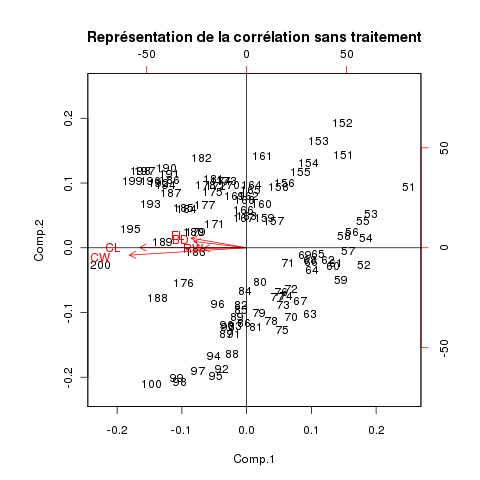
\includegraphics[height = 8cm, width = 8cm]{plots/biplot_acp2_crabs.png}
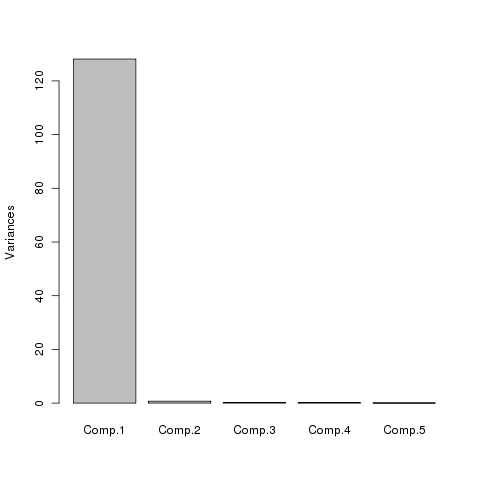
\includegraphics[height = 8cm, width = 8cm]{plots/plot_acp2_crabs.png}\\
Nous pouvons observer sur ce graphique la forte corr\'elation des variables comme vu dans les questions pr\'ec\'edentes.\\ \\
% QUESTION
\textbf{Trouver une solution pour am\'eliorer la qualit\'e de votre repr\'esentation en termes de visualisation des diff\'erents groupes}\\
Pour am\'eliorer la qualit\'e de la repr\'esentation en termes de visualisation, nous avons retir\'e la variable \textit{CL}
des donn\'ees puis nous avons refait une ACP et nous avons repr\'esent\'e les donn\'ees obtenues :
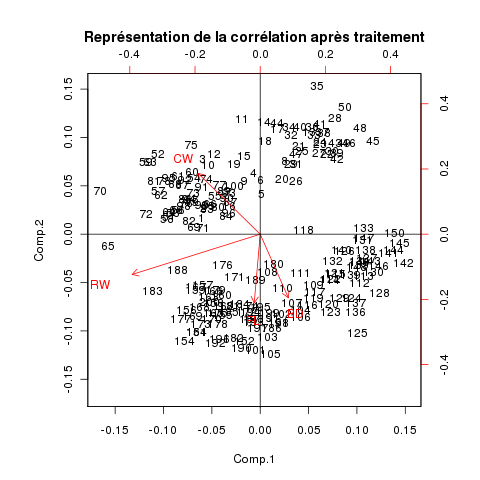
\includegraphics[height = 8cm, width = 8cm]{plots/biplot_acp3_crabs.png}
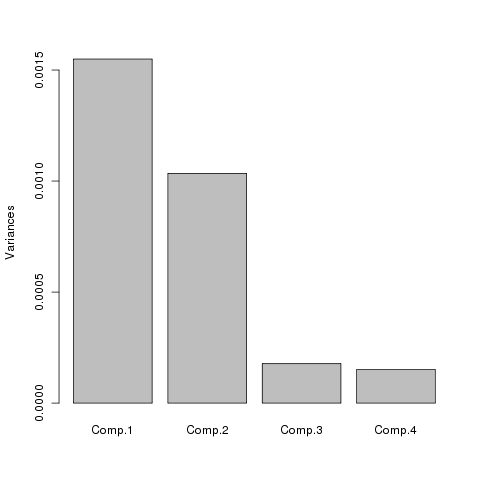
\includegraphics[height = 8cm, width = 8cm]{plots/plot_acp3_crabs.png}\newpage
Nous pouvons remarquer que les variables ne sont plus aussi corr\'el\'ees que pr\'ec\'edemment ce qui nous donne les graphiques suivants
pour diff\'erencier les esp\`eces :\\
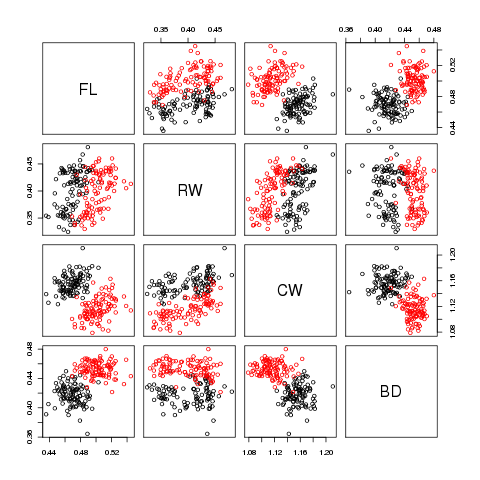
\includegraphics[height = 8cm, width = 8cm]{plots/plot_crabs_sp_2.png}\\
Le graphique pour diff\'erencier les sexes des crabes est :\\
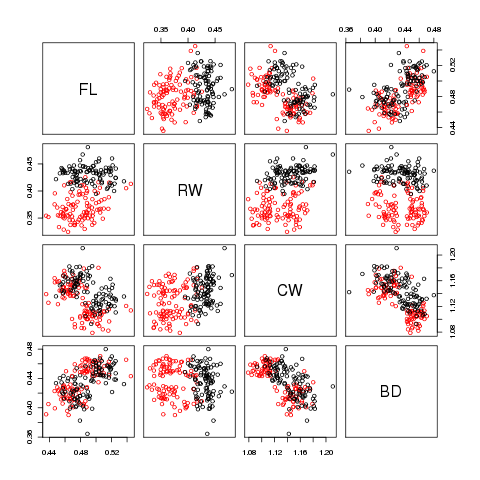
\includegraphics[height = 8cm, width = 8cm]{plots/plot_crabs_sex_2.png}\\ \\
\textbf{Conclusion :}\\
Nous avons pu voir que l'ACP est un outil utile pour repr\'esenter des informations qui auraient \'et\'e difficiles \`a d\'etecter avec
seulement l'utilisation de la statistique descriptive.

\end{document}
